\chapter{Legal and Ethical Challenges of Decentralised Data Environments}
\label{chap:legal}

\begin{tcolorbox}[colback=royallavender!40]
The content of this Chapter has already been partially included in the articles published during this Thesis \citep{esteves_fostering_2022,asgarinia_who_2023,florea_is_2023}.
\end{tcolorbox}

This Chapter discusses the legal and ethical challenges of the impact of data-driven innovation in society, in particular, related to the emergence of PIMS as a service that helps individuals have more control over the processing of their data.
While some studies have recently been published on the intersection of Solid and data protection requirements, as reviewed in Section~\ref{sec:sota_solid_data_protection}, plenty still has to be overcome to have a `legally-aligned' personal datastore.
This interdisciplinary discussion relies on the collaborations fostered through the PROTECT project, and other EU-funded projects described in Section~\ref{sec:projects}, as well as through the participation in the W3C DPVCG work with data protection law experts.

Section~\ref{sec:motivation_legal} describes the emergence of decentralised personal information management systems as a way to give users more control over their personal data and the challenges that still need to be overcome in order to have to a GDPR-aligned personal datastore.

Section~\ref{sec:policies_consent} discusses the usage of OAC policies as a precursor of consent for Solid, which can enable compliance with several GDPR requirements including the transparent information obligations of Articles 13 and 14 and the conditions to obtain valid consent pursuant to Articles 4.11 and 7.

Section~\ref{sec:automation_consent} argues whether the automation of consent can be performed while maintaining the `informed', `freely given', `specific', and `unambiguous' character of GDPR consent.
In particular, the specificity of purposes and processing operations, the distinction between data controllers and recipients, the compatibility of purposes, and the delegation of consent are further analysed through a `legal+tech' approach, relying on GDPR's requirements and on the OAC and PLASMA implementations.

Section~\ref{sec:biomedical_exception} discusses the special requirements of GDPR's special categories of data and research-related exceptions and, in particular, the requirements related to the sharing of health data for biomedical research or for the management of public health.

\section{The emergence of decentralised PIMS}
\label{sec:motivation_legal}

As previously mentioned in Section \ref{sec:def_data_protection_law}, the governance of data flows, and in particular of \textit{personal} data flows, has been a topic of discussion since the early 1970s and 1980s, when the Fair Information Practice Principles (FIPPs) \citep{cate_failure_2006} and Convention 108 \citep{council_of_europe_convention_1981} were first created, to GDPR and subsequent personal data-related regulations being developed in countries such as Brazil or India \citep{bradford_brussels_2019}.
Most of these instruments rely on the existence of an accountable entity that is responsible for establishing the purpose of processing personal data from a natural person, who has rights that must be respected for said processing to be considered compliant with the law.
This model has been the most prevalent since most personal data are stored in large centralised databases under the control of only a certain number of Big tech companies, however, it does not account for cases where the processing is shared among different entities which have distinct purposes or rely on unsuitable legal bases, or the information overload that prevents individuals from actually understanding what they are consenting to \citep{benshahar_more_2014}.
As such, new data governance systems that assist individuals in having more control over their data and trust in data processing services, such as \textit{data cooperatives}, \textit{data trusts}, \textit{data commons} or \textit{personal data sovereignty} schemes, are being proposed \citep{viljoen_relational_2021,craglia_digitranscope_2021} and are even starting to be regulated, such as the new requirements on data intermediation services described in the DGA \citeyearpar{noauthor_regulation_2022}.

In this context, the emergence of decentralised PIMS for the Web, such as the personal datastores model promoted by Solid and studied in this Thesis, has earned many advocates in the last years.
In particular, when it comes to trust, the usefulness and ease of use of digital personal datastores have been proven to be an important factor in increasing citizens' trust in personal data-handling services by allowing them to share their sensitive data for the `public good' while maintaining a sense of control over their data \citep{mariani_explaining_2021}.
Moreover, while these decentralised solutions are not without their faults, as has been shown by blockchain-related scandals in the financial services industry \citep{zetzsche_ico_2019}, their Semantic Web-based counterparts have been gaining a large number of adopters recently as such systems can actually allow its users to choose who can access their data and, therefore, actually shift the power balance in favour of the individuals.
By detaching the storage of data from the data processing services and promoting the usage of Web standards, individuals can move their data between storage providers, use the same data across different services and choose which services and applications best suit their preferences and needs without being locked out of the access to their data \citep{verbrugge_towards_2021,ilves_roadmap_2019}.
This user-managed access to data represents a considerable change from the current \textit{status quo}, where individuals must usually accept an application's privacy policy in order to use it, while personal datastores present the next step towards having an actual negotiation of privacy terms between individuals and data processing entities.
Such systems are also promoted by the EDPS as a mechanism to enable personal data sovereignty where ``Individuals, service providers and applications would need to authenticate to access a personal storage centre'' in an interoperable manner \citep{european_data_protection_supervisor_techdispatch_2021}.
Additionally, the European data spaces initiative launched by the European Commission \citep{european_commission_communication_2020} follows the same spirit by encouraging the development of infrastructures for data holders and data users to share and reuse data across different services while respecting European data protection law.

While personal datastores' developers have as their main banner that data subjects are `controllers' of their data, this view is incompatible with most data protection-related regulations as \textit{``most [...] legal systems are structured around the identification of an accountable entity''} \citep{chomczyk_penedo_selfsovereign_2021} which is given duties in order to ensure that their data processing activities do not affect data subjects' fundamental rights.
In addition, personal data processing activities often involve a complex web of parties that share control of the usage, storage and collection of data for distinct and shared purposes, a fact that makes the compliance with the information requirements described in GDPR's Articles 12 to 14 quite challenging and difficult to implement \citep{lovato_more_2023} -- compliance with such requirements is usually dealt with by providing lengthy and complex notices which are not easy to understand and place a significant burden on data subjects as they have to deal with at least one notice for personal data processing service they use \citep{terpstra_improving_2019,linden_privacy_2020}.
Although these notices usually address the information required by the law, in no way do they fulfil the `informed' character of consent, as prescribed in GDPR's Article 4.11, as it is impossible for data subjects to understand the plethora of terms and conditions of all the personal data handling services that are used nowadays, from smartphone applications to personalised streaming of content, and to give consent in a freely, specific, informed and unambiguous way \citep{mohan_analyzing_2019}.
Beyond consent management, notices are also an inefficient way for data subjects to exercise their rights.

As such, recently, there has been legal work in identifying the different roles and responsibilities that distinct entities occupy in decentralised systems and how said systems can be used to facilitate the exercise of data subjects' rights, fulfil the data protection principles of privacy by design and by default and improve the clarity and transparency of personal data handling processes in contrast to the existing landscape \citep{janssen_personal_2020}, as described in Section~\ref{sec:sota_solid_data_protection}.
Nevertheless, work still needs to be done to align such decentralised systems with the legal requirements, in particular, related to the identification and enforcement of a lawful basis and transparent purpose that justify the access to data.  
Particularly, in this Thesis, the focus is positioned on how to obtain valid consent in Solid, according to the GDPR, while promoting the usage of automation to improve the current information overload felt by data subjects in terms of consent management.
Accordingly, in this Chapter, the introduction of a semantic policy layer, based on the vocabularies described in Chapter~\ref{chap:vocabularies}, for providing the necessary information to obtain informed and valid GDPR consent is studied from a technical and legal angle.

% FROM THE PAPER: In particular, we focus on the processing of health data (considered a special category of personal data under the GDPR) for biomedical research purposes.}

It is likewise important to distinguish between what can be technologically or legally enforced.
Although technically a certain app or service can be restricted to only access certain data, by being allowed to read data from a personal datastore, it can also copy it, even if within a decentralised setting this is not necessary at all.
Thereupon, the realm of law comes into play.
Although the wishes of the data subjects, as stated by the preferences they have stored in their personal datastore, have a role to play in the negotiation of privacy terms between data subjects and data controllers \citep{verborgh_paradigm_2017}, their legal value is still up to debate, as these are quite new technological tools which are still to be argued and tested in the court of law.
\section{Policies as a precursor of consent}
\label{sec:policies_consent}

This Section discusses the usage of OAC policies as a tool to express consent in advance for Solid and how such policies can enable compliance with several GDPR requirements including the transparent information obligations of Articles 13 and 14.
As such, these policies come as a solution to overcome the shortcomings of Solid's access control mechanism when it comes to dealing with GDPR's information requirements.
Moreover, by enabling the communication of this information, policies can be used as a tool to fulfil the conditions to obtain valid consent under Articles 4.11 and 7 of the GDPR.

\subsection{Distinguishing consent from access control}
\label{sec:distinction}

It is important to make a distinction between the legal notion of giving consent and the technical means used to grant an app, service or user-authorised access to a resource stored in a decentralised personal datastore such as a Solid Pod.

As previously discussed in Section~\ref{sec:sota_solid_access_control}, Solid Pods are decentralised, permission-based data storage environments, by default.
This means that in the absence of a tangible authorisation, resources cannot be accessed by apps or users.
Authorisations can then be provided in a direct and indirect way by accepting requests from apps as they are being received or by setting the rules of access in advance, respectively.

From GDPR's viewpoint, user authorisation is not always required for the processing of personal data, but it also might not be enough for entities to process personal data in a lawful manner in such decentralised settings.
In the first case, it might be \textit{unnecessary} as there are other legal bases in GDPR's Article 6.1 which can be used, beyond consent, that do not involve an active choice being made by the data subject, such as the performance of a contract --Article 6.1(b)-- or the legitimate interests of the data controller --Article 6.1(f)-- \citep{kranenborg_article_2014}.
Taking the former as an example, there is no need to have the consent of the data subjects to access personal data when they have entered into a contract with the data controller and access to said data is necessary for the performance of said contract \citep{european_data_protection_board_guidelines_2019}.
Moreover, if indeed the access is based on the consent of the data subject, then the current status quo of access control in Solid --whether being the WAC or the ACP authorisation mechanisms-- is not enough for obtaining valid consent according to the GDPR, as in Article 4.11 valid consent is described as being a \textit{``freely given, specific, informed and unambiguous indication of the data subject’s wishes''} \citeyearpar{noauthor_regulation_2016}. 

By comparing both the legal and the technical requirements, described in the previous paragraphs, it is possible to arrive at two sets of problematic cases:
\begin{itemize}
    \item[(i)] instances when app providers have a valid legal basis beyond consent to have access to the data, but do not have access to said data as no permission-based authorisation, granted by the data subject, is stored in the Pod; and
    \item[(ii)] instances when app providers use consent as a ground for lawfulness, however, the authorisation available on the Pod does not fulfil the conditions for valid consent according to Articles 4.11 and 7.
\end{itemize}

In this Thesis, the second cluster of cases is explored by discussing whether the introduction of fine-grained access control policies, modelled with OAC, is enough for obtaining valid consent.

\subsection{Introducing OAC policies in the Solid ecosystem} % Introducing OAC policies in the Solid ecosystem: from notice to automated consent
\label{sec:oac_notice_automation}

In addition to a lawful basis for processing, Article 5.1(a) states that personal data should be \textit{``processed [...] in a transparent manner in relation to the data subject''} \citeyearpar{noauthor_regulation_2016}.
The information obligations described in Articles 12 to 14 depict the required information that data subjects must be provided with, regardless of the chosen legal basis, in order to have transparent information regarding the processing of their personal data.
This means that data subjects always have the right to have access to this information, while data controllers are always obliged to provide it, even if the legal basis for processing personal data is not consent.
Additionally, Recital 59 provides that \textit{``Modalities should be provided for facilitating the exercise of the data subject’s rights [...] free of charge [...]''}.
In this context, OAC policies can serve as a modality that enables the data subjects' right to information regarding the processing of their personal data.
In particular, OAC-based agreements stored on Solid Pods, such as the one depicted in Listing~\ref{list:oac_agreement}, resulting from the matching of user offers and data requests, \beatriz{described in detail in Chapter XX, } are thus accessible to data subjects and can be used by them to easily understand whether the specific conditions for accessing data, set on the agreement, vary from their personal preferences stored in the Pod in the form of OAC-based preferences and requirements.

The specific privacy terms that need to be provided by data controllers are specified in GDPR's Articles 13 and 14 and detailed in Table~\ref{tab:GDPR_privacy_terms} as informational items I1 to I19.
As can be checked in Figure~\ref{fig:oac_diagram} and Table~\ref{tab:profile_classes}, the OAC profile provides concepts to express personal data types, legal basis, recipients, purposes for processing, processing operations and the identity of the data controllers accessing the data. 
This leaves out some elements noted in Article 13.1, namely the controller's contact details and its representative, the DPO's contact details, the legitimate interests of the data controller or third party recipient, if the used legal basis is grounded on Article 6.1(f), and information about the transfer of data to third countries or international organisations.
Moreover, Article 13.2, in order to ensure fair and transparent processing, also states that data subjects should be informed about the retention period of the data, the existence of data subject rights, statutory or contractual obligation details if the provision of data is a requirement to enter into a contract or a statutory obligation, including the possible consequences of failing to provide such data, and the existence of automated decision-making.

If the user’s policies do not include all these necessary elements, or if there are discrepancies between them and the data access request, then the data subject should be notified about this information at the time of the data request.
In Solid, as previously stated in Section~\ref{sec:distinction}, access can be granted by (i) accepting requests when starting to use a new application or by (ii) setting the access rules in advance.
In the first case, this is done through an authorisation dialogue, such as the examples provided in Figure~\ref{fig:authorisation-dialogue}, and, in the second, through a Pod management app, such as Inrupt's PodBrowser\footnote{{\url{https://docs.inrupt.com/user-interface/podbrowser/} (accessed on 21 December 2023)}} in Figure~\ref{fig:podbrowser} or Penny\footnote{{\url{https://penny.vincenttunru.com/} (accessed on 21 December 2023)}} in Figure~\ref{fig:penny}.
Figure~\ref{fig:css} illustrates the authorisation dialogue related to the Community Solid Server (CSS)\footnote{{\url{https://communitysolidserver.github.io/CommunitySolidServer/7.x/} (accessed on 21 December 2023)}} and Figure~\ref{fig:ess} the Inrupt's Enterprise Solid Server (ESS)\footnote{{\url{https://www.inrupt.com/products/enterprise-solid-server} (accessed on 21 December 2023)}} Pod and identity providers.
While ESS's dialogue includes some information on the purposes for access and CSS's on the specific types of access being provided, as is visible through the Figures, both dialogues do not include all the elements previously discussed for the user to be able to provide informed consent.

\begin{figure*}[htp]
    \caption[Screenshots of the authorisation dialogues of existing Solid servers (CSS and ESS).]{Screenshot of the authorisation dialogue of the}
    \label{fig:authorisation-dialogue}
    \centering
    \subfigure[Community Solid Server]{
        \fbox{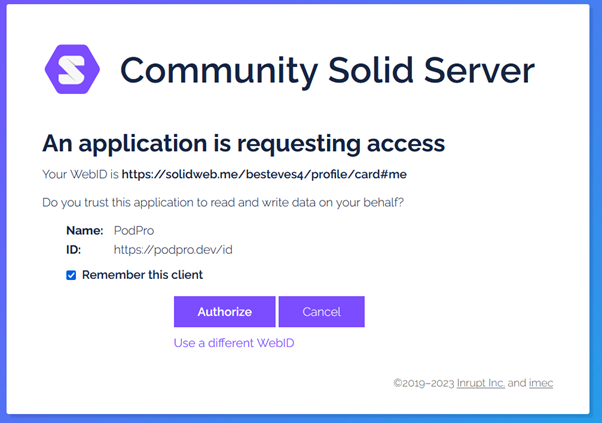
\includegraphics[width=0.4\linewidth]{figures/chapter-5/css.png}}
        \label{fig:css}
    }
    \qquad
    \subfigure[Enterprise Solid Server]{
        \fbox{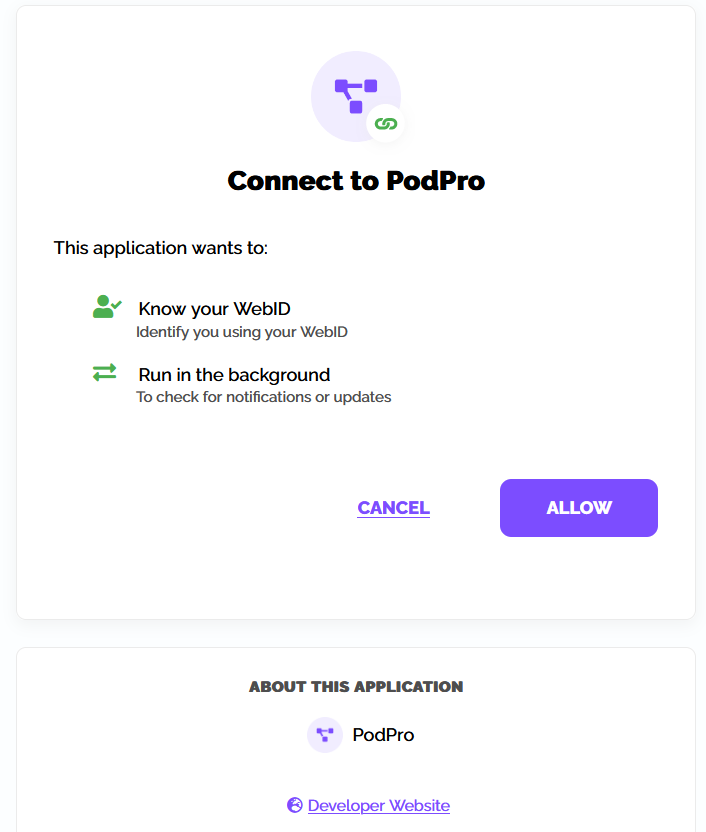
\includegraphics[width=0.4\linewidth]{figures/chapter-5/ess.png}}
        \label{fig:ess}
    }
\end{figure*}

\begin{figure}[htp]
    \centering
    \fbox{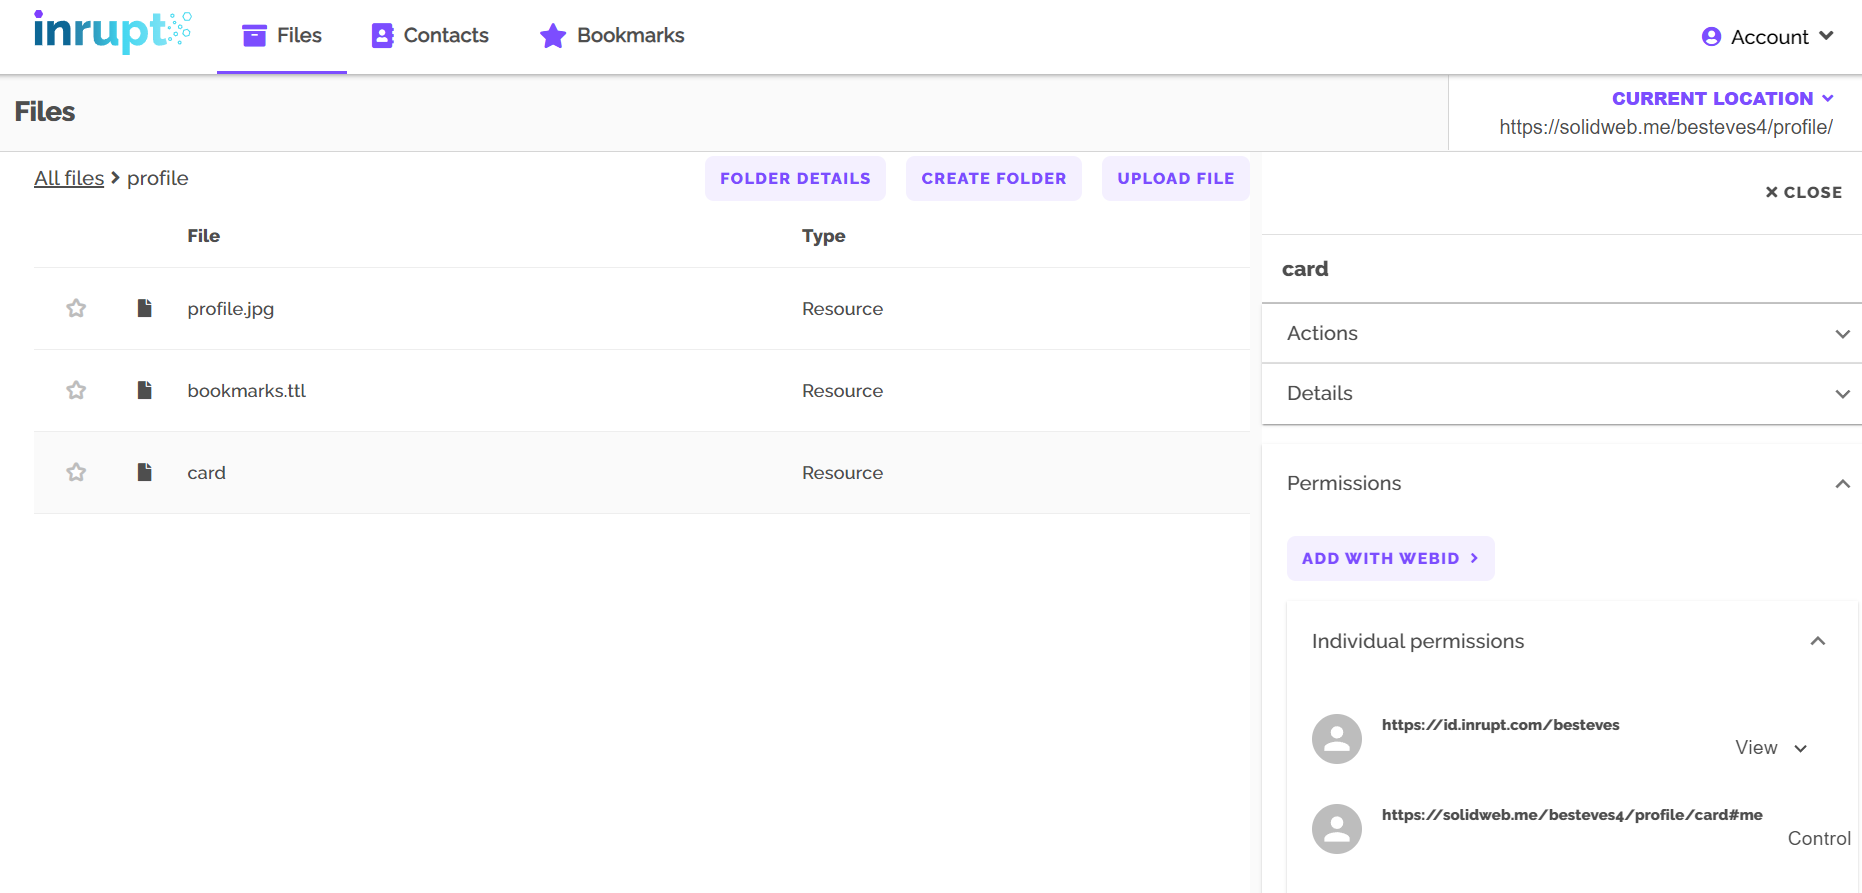
\includegraphics[width=0.9\linewidth]{figures/chapter-5/podbrowser.png}}
    \caption{Screenshot of Inrupt's PodBrowser app to manage data and access grants.}
    \label{fig:podbrowser}
\end{figure}

\begin{figure}[htp]
    \centering
    \fbox{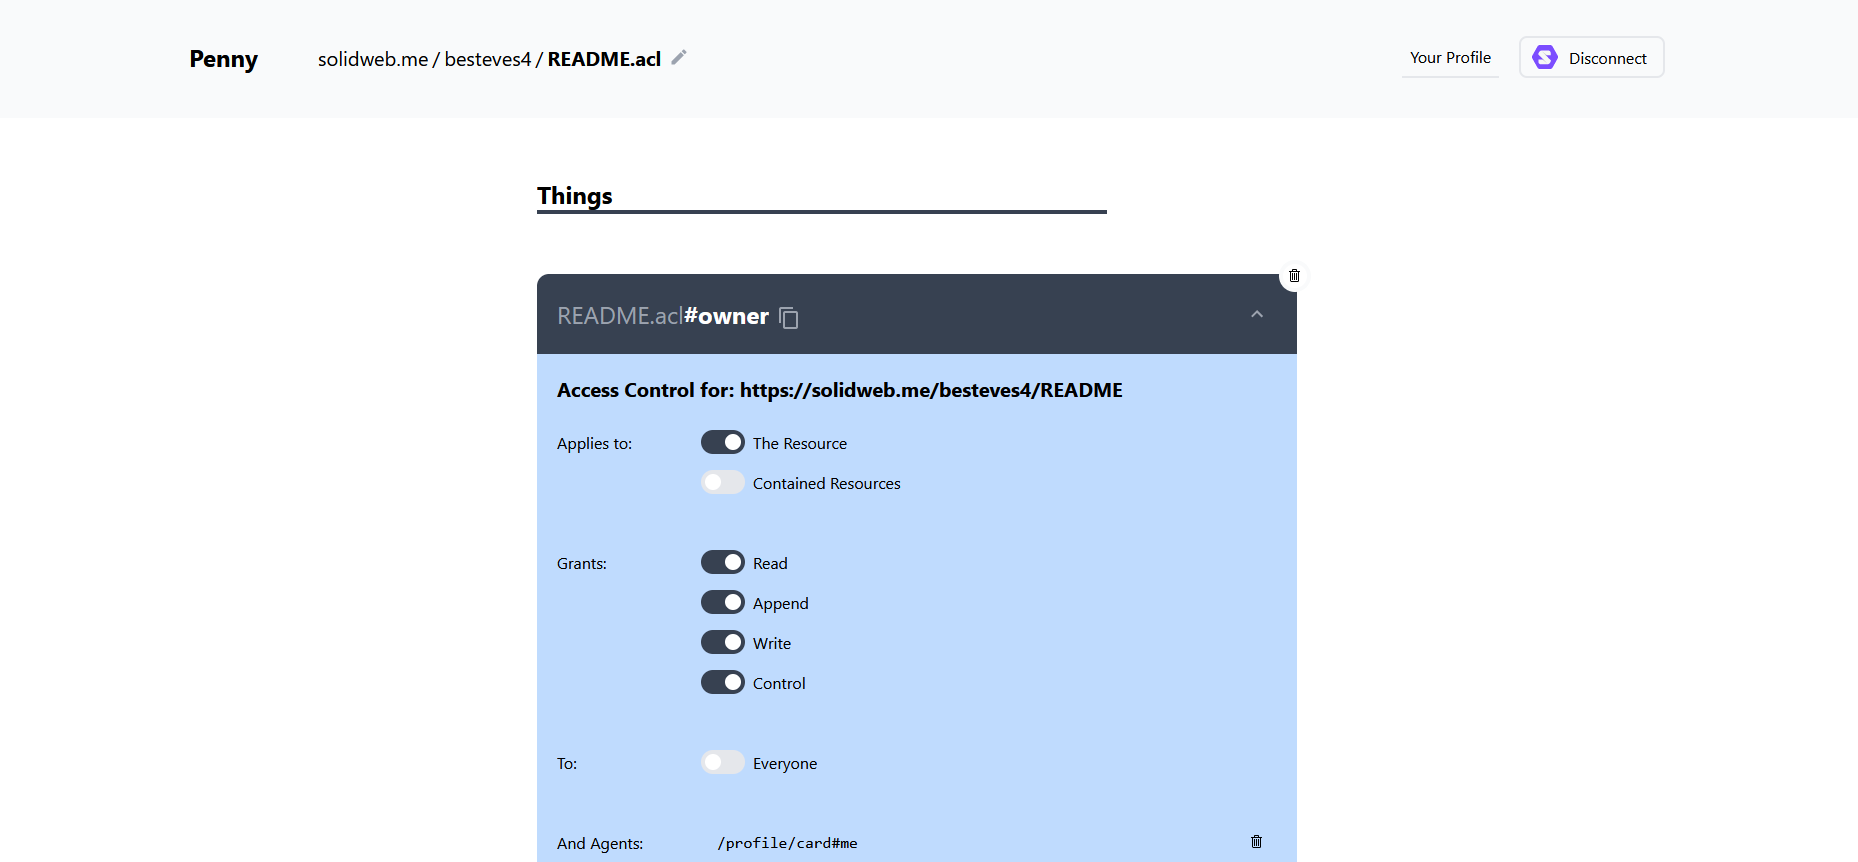
\includegraphics[width=0.9\linewidth]{figures/chapter-5/penny.png}}
    \caption{Screenshot of Penny app to manage data and access grants.}
    \label{fig:penny}
\end{figure}

Furthermore, two more legal challenges should be considered regarding the information obligations set out in the GDPR.
The first relates to how the information is presented to the data subject as GDPR Article 12 states that data controllers have an obligation to provide this information \textit{``in a concise, transparent, intelligible and easily accessible form, using clear and plain language''} \citeyearpar{noauthor_regulation_2016}.
As such, while the user's policies, others' requests and data access agreements can be easily accessed by data subjects if stored in Solid Pods, the implementation of interfaces to display the result of the policy matching process, especially the information that was previously unknown by the subject, might also be necessary to fully fulfil the requirements of Article 12 in ensuring that data subjects have read and understood this information.

The second challenge is related to the timing of the notification, as Articles 13 and 14 set different rules which depend on whether the data collection is done directly from the data subject or another entity.
As the GDPR does not directly mention data intermediary services, there is a gap that should be further explored to understand which Article applies in the Solid context.
On one hand, if the Pod provider is deemed a data controller, then the personal data is not directly collected from the data subject \citep{pandit_making_2023} and Article 14 applies, meaning that the data subject must be informed \textit{``at the latest at the time of the first communication to that data subject''} \citeyearpar{noauthor_regulation_2016}.
Access requests to Solid Pods can be considered to be communications with data subjects, and as such, at the time of the request, the information requirements should be fulfilled.
On the other hand, if the Pod provider is not thought to be a data controller, i.e., it is simply considered a piece of software used by the data subject, then the data is directly captured from the data subject and Article 13's requirements must be fulfilled at the time when said data is obtained.
Regardless, in both interpretations, the data subjects must be notified at the latest in the instant when the requests reach the data subjects' Pod.

%Both existing options to provide access in Solid can take distinct forms, as clearly stated by Figures~\ref{fig:authorisation-dialogue}, \ref{fig:podbrowser} and \ref{fig:penny}, also depending on the access control specification implemented in the server where the Pod is stored, since servers only have to comply with one access control protocol, i.e., WAC or ACP, as described in Section~\ref{sec:sota_solid}.

%FROM THE PAPER: The outcome of the matching exercise is a mapping between the user’s policies and the specifics of the request for accessing the data, emphasizing the differences between the two. This process can lower the burden of data subjects in reading and comprehending the information related to the processing of their personal data.

Additionally, the informed character of consent is only one of a series of requirements that must be met in order to obtain valid consent. 
After being informed, data subjects must state their preferences \textit{``by a statement or by a clear affirmative action''} \citeyearpar{noauthor_regulation_2016} which signifies their agreement with the handling of their personal data.
Moreover, EDPB's and WP 29's guidelines on consent \citep{european_data_protection_board_guidelines_2020,article_29_data_protection_working_party_opinion_2011,article_29_data_protection_working_party_article_2018} further develop the freely given, specific, informed and unambiguous characters of consent.
Among the discussed topics, these entities' guidelines state that consent must be granular, the data subjects must be aware of the consequences of refusing to consent and the distinct purposes for processing data must not be tied together.
Thus, simply accepting an access request does not necessarily signify consent according to the GDPR.

\subsection{Expressing consent in advance through OAC policies}
\label{sec:consent_advance}

The GDPR does not forbid the expression of consent in advance.
In fact, Recital 32 mentions that \textit{``Consent should be given by a clear affirmative act [...], such as by a written statement, including by electronic means, [...]. This could include ticking a box when visiting an internet website, choosing technical settings for information society services or another statement or conduct which clearly indicates in this context the data subject’s acceptance of the proposed processing of his or her personal data''} \citeyearpar{noauthor_regulation_2016}.
Nevertheless, in order for consent to be valid under the GDPR jurisdiction, it must be specific even for circumstances that may not have already happened \citep{kosta_consent_2013} and the data controllers must be able to demonstrate that \textit{``the data subject has, by active behaviour, given his or her consent to the processing of his or her personal data and that he or she has obtained, beforehand, information relating to all the circumstances surrounding that processing, in an intelligible and easily accessible form, using clear and plain language, allowing that person easily to understand the consequences of that consent, so that it is given with full knowledge of the facts''}, as stated in Case C-61/19 held in 2020 at the European Court of Justice \citeyearpar{noauthor_orange_2020}.
As such, in this Section, the usage of OAC policies to express the required GDPR terms to have valid consent are further explored. 
 
The automation of consent on the Web is not a new idea.
As a matter of fact, the Do Not Track (DNT)\footnote{\url{https://www.eff.org/issues/do-not-track} (accessed on 28 January 2024)} initiative and the previously described P3P are two examples in this respect.
Although none of these solutions have succeeded in being consumed at a large scale, they can be illustrative use cases of what to do -- and do not do -- while developing a system for Web consenting. 
The DNT initiative focused on blocking the ad-tech industry from tracking users based on their online behaviour by sending a signal from the users' browser to all Web pages they visited with the preference to not be tracked, similarly to the right to object asserted in GDPR Article 21, however it failed due to the lack of browser adoption and enforcement mechanisms \citep{kamara_not_2016}.
Similarly, the P3P initiative allowed Web pages to \textit{``express their privacy practices in a standard format that can be retrieved automatically and interpreted easily by user agents''} and \textit{``enable an expanded ecosystem in which web sites would consistently inform web user agents of personal data collection intentions and web users would configure their individual user agents to accept some practices automatically [...]''} \citep{cranor_platform_2002}.
However, one of P3P's main drawbacks was the lack of consistency between human and machine-readable privacy notices communicated to users \citep{cranor_web_2002}, a challenge which can also be attributed to Solid as the information presented to users in consent dialogues is not aligned with the authorisation statements stored in Solid Pods.
Moreover, WP 29 also stated that P3P had the capability of misleading data controllers into believing that they could be discharged of certain obligations as long as data subjects had already agreed to the processing of their data \citep{article_29_data_protection_working_party_article_2014}, an issue which can also very easily be relevant for the Solid ecosystem.

Nevertheless, Solid differs from P3P in the sense that it provides its users with a decentralised storage unit equipped with a permission-based access control mechanism, i.e., access to data is only provided in the presence of an authorisation for a particular application or user.
Furthermore, in such decentralised systems there is no need to transfer or make copies of data as access can be provided on demand to any user or application through its authorisation and authentication mechanisms, removing the need for such entities to keep copies of data in their own servers.
Said mechanisms can also serve as the starting point to keep access and usage logs in Solid Pods, which can be used by users and by external auditing entities to check whether Web services are using data according to their announced policies.
As such, users will have a more transparent overview of how their data is being used, which comes as an improvement over P3P’s lack of consistency and policy enforcement -- \textit{``no enforcement action followed when a site's policy expressed in P3P failed to reflect their actual privacy practices''} \citep{cranor_platform_2002} --, the main issues that led to its failure.
What's more, as previously stated in Section \ref{sec:sota_solid_data_protection}, there is ongoing research on the modelling of usage control policies \citep{akaichi_gucon_2023} and enforcement mechanisms for Solid \citep{slabbinck_rulebased_2023}.

% FROM PAPER: In a rather recent development, the Commissioner for Justice and Consumers, Didier Reynders, launched a reflection on how \replaced{better to}{to better} empower consumers to make effective choices regarding tracking-based advertising models \textls[-15]{({\url{https://commission.europa.eu/live-work-travel-eu/consumer-rights-and-complaints/enforcement-consumer-protection/cookie-pledge\_en}, accessed on 19/11/2023})}. The problem that it tries to solve is similar to the difficulties around accessing content in Solid Pods. 

The usage of pre-configured choices is also discussed in Recital 66 of Directive 2009/136/EC, the successor of the ePrivacy Directive \citeyearpar{noauthor_directive_2002}, which states that \textit{``Third parties may wish to store information on the equipment of a user, or gain access to information already stored, for a number of purposes, ranging from the legitimate (such as certain types of cookies) to those involving unwarranted intrusion into the private sphere (such as spyware or viruses). [...] Where it is technically possible and effective, [...] the user’s consent to processing may be expressed by using the appropriate settings of a browser or other application''} \citeyearpar{noauthor_directive_2009}.
This is also reflected on a few national implementations of the ePrivacy Directive that allow the indication of consent via technical means, e.g., Romania's Legea 506/2004 states that \textit{``the subscriber or user can use the settings of the internet browsing application or other similar technologies to delete stored information or to deny access to such information to third parties''} \citeyearpar{noauthor_legea_2004}.
However, the utility of browser settings to express consent is being challenged as recently the data protection authority in Finland ruled that \textit{``instructing website users to accept or decline to the use of cookies through browser settings does not constitute active and explicit consent under the GDPR''} \citep{fich_finland_2021}.
Nonetheless, several technical solutions to signal users' preferences have been emerging recently, e.g., the Global Privacy Control (GPC) \citep{global_privacy_control_gpc_2021} or the Advanced Data Protection Control (ADPC) \citep{human_advanced_2021} \textit{`privacy signals'}, which are still lacking adoption due to a lack of standardisation and legal approval towards the fulfilment of ePrivacy requirements \citep{santos_how_2023}.

In the next Section, the building blocks for the expression of consent in advance are explored in detail, with a reflection on how Solid can be adapted to fulfil legal requirements. 
\section{Can consent be automated?}
\label{sec:automation_consent}

To discuss consent automation, first one should look into the rationale of why it is such an important requirement in personal data protection law.
As per \cite{jarovsky_improving_2018}, the main rationale behind consent is to retain human autonomy and to enable data subjects to have agency regarding the processing of their data.
To achieve that, data subjects must (i) comprehend the circumstances that surround the processing of their data, (ii) decide which is their optimal choice among a variety of options, and (iii) express their choice, while knowing that they can change it at any point in the future.
However, if there are no technical and/or organisational measures in place to preserve individual autonomy in this process, meaningful, freely given consent cannot be achieved due to \textit{``issues of cognitive limitations, information overload, information insufficiency, lack of intervenability and lack of free choice''} \citep{jarovsky_improving_2018}.
\cite{solove_privacy_2012} also outlined a few shortcomings in the self-management of privacy, distinguishing between cognitive limitations related to human decision-making abilities and structural limitations that prevent an adequate cost-benefit analysis of consenting to simultaneous personal data processing activities. 
As such, presenting Solid users with a consent dialogue with the result of the matching for each access request that comes in will result in similar scalability issues for the users \citep{mcdonald_cost_2008}.

One possible solution to the previously identified consent-related issues is to automate some aspects of giving consent \citep{baarslag_automated_2017}.
However, this solution has often been criticised due to the complexity surrounding current personal data processing activities on the Web, which might compromise the validity of consent \citep{jarovsky_improving_2018,solove_murky_2023}.
Consenting is context-dependent and encompasses weighing the risks, likelihood of harms and benefits of several variables involved in a personal data processing activity.
As such, it is difficult to imagine how an automated system can weigh all the arguments in favour and against the processing of personal data, while maintaining the interests and autonomy of the data subject at the center of the decision making algorithm.

Thus, in this Section, the setting of OAC user policies in advance and the matching of such policies with requests for data access is analysed to check if such a system is sufficient to comply with the legal requirements for expressing valid consent.
Consenting is usually a binary choice -- the data subject either agrees with the conditions set by the data controller to process their data or they do not.
Nevertheless, different privacy laws implement this choice in distinct manners: in the United States the `opt-out' choice predominates, i.e., \textit{``organizations post a notice of their privacy practices and people are deemed to consent if they continue to do business with the organization or fail to opt out''}, while in the EU the `opt-in' option prevails, i.e., \textit{``people must voluntarily and affirmatively consent''} \citep{solove_murky_2023}.
As such, the latter involves (i) the data controller requesting consent and (ii) the data subject accepting or rejecting it.
If users set their policies in advance, this order is inverted.
Even though the GDPR does not regulate the interaction between data subjects and software to assist them in expressing consent, as previously mentioned, Recital 32 \citeyearpar{noauthor_regulation_2016} suggests the usage of \textit{``technical settings''} to indicate \textit{``acceptance of the proposed processing of his or her personal data''}.

Moreover, two levels of automation, both triggered by a data request, can be considered: (i) the result of the matching, between user policies and data request, is presented to the user for him/her to consent, or (ii) access to data is given automatically if the data request matches with the user's policies.
The former -- the consent dialogue, based on the policy matching algorithm -- improves the transparency of the processing activity and helps the data subject to make an informed choice, while the latter assists with the issues related to information overload and scalability.

% TODO: explain function creep and right to informational self-determination in the footnotes and add references
In the next Sections, the specific character of consent is going to be analysed to understand whether OAC can be used to automate access to data in Solid Pods in a GDPR-aligned manner.
According to Article 4.11 \citeyearpar{noauthor_regulation_2016}, consent must express a specific \textit{``indication of the data subject’s wishes''} that \textit{``signifies agreement to the processing of personal data relating to him or her''}.
However, the wording ``indication of wishes'' is rather vague in the sense that such wishes might be related to the categories of personal data, the purpose for processing, the processing operations, the identity of data controller(s) and/or third party recipients, or their interconnection.
Moreover, the European Court of Justice mentions in Case C-61/19 Orange Romania \citeyearpar{noauthor_orange_2020} states that the data subject’s wishes \textit{``must relate specifically to the processing of the data in question and cannot be inferred from an indication of the data subject’s wishes for other purposes''}.
The EDPB also included guidance on the specificity of consent in its consent guidelines \citep{european_data_protection_board_guidelines_2020}, in particular related to (i) using purpose as a safeguard against `function creep'\footnote{\cite{koops_concept_2021} defines `function creep' as \textit{``an imperceptibly transformative and therewith contestable change in a data-processing system's proper activity''} or, in simpler terms, \textit{``the expansion of a system or technology beyond its original purposes''}.}, (ii) the granularity of consent requests, and (iii) the requirement to provide information related to consent separately from other data processing matters.
Moreover, pursuant to Recital 42 \citeyearpar{noauthor_regulation_2016}, for consent to be informed, the data subject should be aware of, at least, the purpose for the personal data processing and the identity of the controller(s). 
However, the level of detail in which the purpose must be described is not further prescribed in the regulation.
According to \cite{kosta_consent_2013}, the specificity of consent is fulfilled when the relation between personal data and its processing, as well as all other conditions surrounding the processing activities, are explained.
Furthermore, consenting should be as specific as needed for safeguarding the data subject's right to informational self-determination\footnote{The right to informational self-determination was first formulated in German law and it has had a profound impact in European data protection law as it asserts that an individual should have the authority \textit{``to decide fundamentally for herself, when and within what limits personal data may be disclosed, [...]''} \citep{vivarelli_crisis_2020}.}.
As such, the following analysis will be focused on the purpose of processing personal data, as well as on the identity of the data controller, and how they relate to the specific character of consent.

\subsection{Distinguishing the processing operation from the purpose for processing}
\label{sec:processing_purposes}

The GDPR explicitly mentions that not only the purpose but also the processing operation needs to be specific to have valid consent.
Article 6.1(a) \citeyearpar{noauthor_regulation_2016} states that \textit{``Processing shall be lawful only if [...] the data subject has given consent to the processing of his or her personal data for one or more specific purposes''}, while Recital 43 \citeyearpar{noauthor_regulation_2016} pinpoints that \textit{``Consent is presumed not to be freely given if it does not allow separate consent to be given to different personal data processing operations despite it being appropriate in the individual case''}.
Hence it is important to distinguish between both.
While processing operations refer to the actions performed over data -- personal data in the case of GDPR --, the purpose expresses the motive or objective of the data controller for processing personal data.
This also means that several processing operations might be needed to reach a purpose and, on the other hand, distinct purposes can be reached through the same operation, with use of data being a case in point since it has a very broad scope.
As such, \textit{``collection, recording, organisation, structuring, storage, adaptation or alteration, retrieval, consultation, use, disclosure by transmission, dissemination or otherwise making available, alignment or combination, restriction, erasure or destruction''} are examples of processing operations set out on Article 4.2 \citeyearpar{noauthor_regulation_2016}, while Article 5.1(e) \citeyearpar{noauthor_regulation_2016} mentions purposes such as \textit{``archiving purposes in the public interest, scientific or historical research purposes or statistical purposes''}.
Moreover, the distinction between both is also made explicit in Recital 32, which states that \textit{``Consent should cover all processing activities carried out for the same purpose or purposes. When the processing has multiple purposes, consent should be given for all of them''}.
As such, this provision can be interpreted as follows: (i) if a processing operation is used to reach more than one purpose, then consent must be obtained for each purpose, and (ii) if multiple processing operations are needed to reach a single purpose, then consent must be obtained for each processing operation.

Moreover, WP 29, in its opinion on the definition of consent, affirmed that \textit{``There is a requirement of granularity of the consent with regard to the different elements that constitute the data processing: it can not be held to cover `all the legitimate purposes' followed by the data controller''} \citep{article_29_data_protection_working_party_opinion_2011}, i.e., consent should be specific in relation to a purpose.
The relation between processing operations and purposes is also further commented on by WP 29 on these guidelines -- \textit{``it should be sufficient in principle for data controllers to obtain consent only once for different operations if they fall within the reasonable expectations of the data subject''} \citep{article_29_data_protection_working_party_opinion_2011}, however no further guidance is given on what constitutes `reasonable expectations of the data subject'.
These can be identified, for instance through user studies, however the result of such studies would only be statistically relevant to the average data subject and not to the particular data subject who has to give consent.
Additionaly, the contextual integrity theory of privacy developed by Helen Nissenbaum \citep{nissenbaum_privacy_2004} could also be applied to determine the contextual nature of the processing operation.
Nissenbaum states that privacy should be considered as a right that the individual has over the appropriate, context-based flow of their personal information according to context-specific social norms.
As such, the context and norms governing the exchange of personal data should be used to calculate whether the data subject's given consent is specific or not.
% TODO: develop more on the contextual integrity theory of privacy developed by Helen Nissenbaum
On the other hand, there is no clear guidance on what should be the granularity of the processing operations.
Furthermore, these guidelines also provide an example of how consent fails to be specific -- data that is collected for the purpose of providing movie recommendations cannot be used to provide targeted advertisements as the former is more specific than the latter.

However, in a later guidance document, WP 29 also mentions that there are no tools to assess the specificity of data processing elements such as the processing operation or the purpose
\citep{article_29_data_protection_working_party_article_2016}.
Furthermore, in its opinion on electronic health records \citep{article_29_data_protection_working_party_working_2007}, WP 29 had already advanced that \textit{```Specific' consent must relate to a well-defined, concrete situation in which the processing of medical data is envisaged. Therefore a `general agreement' of the data subject e.g. to the collection of his medical data for an EHR and to subsequent transfers of these medical data of the past and of the future to health professionals involved in treatment would not constitute consent''}.
This document also reasons that if the purpose for processing changes at some point in time, then the data subject must be notified to re-consent to the new personal data processing activity and provided with information related to the repercussions of rejecting to consent to such changes.

At this point, it can be discussed whether any change in the purpose, however small, means that consent must be given again by the data subject.
Perhaps in the case of a minor change, re-consent could be considered unnecessary, however, the criterion to measure such a change is not clearly defined in the law. 
As such, it is essential to analyse the matching of offers and requests, for access to data stored in Solid Pods, to understand if the specific character of consent is respected.
A policy matching algorithm based on OAC, \beatriz{such as the one detailed in Chapter XX}, functions on the basis of subsumption between the data requests and the user policies defined in advance.
Thus, by hypothesis, user policies can be broader than data requests, which can be used to doubt the specificity of the consent.
However, since OAC policies can also include the usage of prohibitions, these can be used to narrow the scope of the data subject consent, making it more specific.

%FROM THE PAPER: The reasoner that implements the matching transforms a preference, expressed through a positive statement (the purpose)\added{,} and one or more negative ones (the prohibitions) into a choice between the available options as it \replaced{materializes}{materialises} the preferences and produces legal effects towards third parties (the data controller).
\section{Special categories of data and research exceptions}
\label{sec:biomedical_exception}

As discussed in preceding Sections, the stringent requirements for obtaining consent under the GDPR place significant burdens on data subjects.
Requiring separate agreements for each app provider and for each specific purpose leads to repetitive consent requests.
In the biomedical field, individuals may have less involvement in decision-making regarding their data compared to other sectors -- the benefits from participation in biomedical research are often not immediate and may not directly impact the individual's personal circumstances.
Consequently, individuals may be less inclined to make the effort of checking their Pod for new requests, reading information notices, and accepting/rejecting access requests, compared to sectors like information society services which include social media and streaming services.
As such, in the context of research, various provisions indicate a more flexible approach to consent requirements or even suggest moving away entirely from reliance on consent.

Recital 33 \citeyearpar{noauthor_regulation_2016} states that broad consent is permissible for research purposes under specific conditions -- \textit{``data subjects should be allowed to give their consent to certain areas of scientific research when in keeping with recognised ethical standards for scientific research''} and while having the \textit{``opportunity to give their consent only to certain areas of research or parts of research projects''}.
However, the terms `areas of research' or `parts of research projects' are domain-specific concepts that are not further defined in the GDPR.
The Global Alliance for Genomics and Health\footnote{\url{https://www.ga4gh.org/} (accessed on 9 March 2024)} develops distinct components and processes for health data sharing, including the Data Use Ontology (DUO)\footnote{\url{http://purl.obolibrary.org/obo/duo} (accessed on 9 March 2024)}, a vocabulary that can be used to describe data use conditions and limitations for research data generated in the health, clinical and biomedical domain \citep{lawson_data_2021,rehm_ga4gh_2021}.
While such vocabulary contains concepts of health-related research purposes, links to other ontologies with disease taxonomies, and incorporates concepts for modeling projects and obligations related to data usage, e.g., need for ethical approval, collaboration with the study's investigator, or the obligation to return the study's results, it does not take into consideration data protection-related requirements, e.g., legal grounds for processing.
% TODO: connect with the DUODRL chapter

However, this provision outlined in Recital 33 \citeyearpar{noauthor_regulation_2016} is not legally binding, is not mirrored in the actual text of the GDPR and it was strictly interpreted by the EDPS in its opinion on data protection and scientific research \citep{european_data_protection_supervisor_preliminary_2020}.
Furthermore, while the EDPS asserts that Recital 33 does not supersede the provisions mandating specific consent, it also suggests an assessment based on the data subject's rights, the sensitivity of the data, the nature and objective of the research, and relevant ethical safeguards. Concurrently, the EDPS also notes that if purposes cannot be precisely specified, data controllers could compensate by enhancing transparency and implementing safeguards.
Outside of the EU, the UK government advocated for an influential role for broad consent in medical research within its proposal to amend the UK's Data Protection Act \citep{uk_government_consultation_2022}.
This proposal was generally well-received, though some concerns were expressed regarding its potential for ambiguity and possible misuse.

Furthermore, the European Commission has proposed a regulation instrument for the health data domain, the European Health Data Space \citeyearpar{noauthor_proposal_2022}, which aims to depart from relying on consent for the secondary use of personal data in biomedical research.
According to this proposal, a `data holder', or a \textit{``any natural or legal person, which is an entity or a body in the health or care sector, or performing research in relation to these sectors [...] who has the right or obligation [...] to make available, including to register, provide, restrict access or exchange certain data''} \citeyearpar{noauthor_proposal_2022}, is mandated to disclose both personal and non-personal data under specific conditions and for a limited set of purposes, including scientific research (Article 34.1(e) \citeyearpar{noauthor_proposal_2022}), without requiring the consent of the data subject.
Additionally, Article 33.5 of the EHDS proposal \citeyearpar{noauthor_proposal_2022} appears to override national laws mandating consent by stipulating that \textit{``where the consent of the natural person is required by national law, health data access bodies shall rely on the obligations laid down in this Chapter to provide access to electronic health data''}.
The final version of this proposal, including the role of consent and its scope (broad or specific), is yet to be determined.
However, this proposal has drawn criticism from both the EDPB and EDPS in a joint opinion document, which calls for further clarification on how national laws requiring consent will interact with the proposed European legislation \citeyearpar{noauthor_edpbedps_2022}.

Biomedical research presents challenges within the GDPR due to its unique combination of a stringent regulatory framework, as it involves processing health data, which falls under the GDPR's special categories of data, alongside a set of exemptions designed to facilitate research due to its societal significance.

\subsection{A stricter regime for health data processing}
\label{sec:stricter_regime}

GDPR's Article 9.1 \citeyearpar{noauthor_regulation_2016} prohibits the processing of special categories of data, including health data.
However, there are ten exceptions to this rule, one of which is explicit consent from the data subject.
Nevertheless, the term `explicit' lacks clarity, as it's unclear what distinguishes it from `regular' consent, which requires a clear affirmative action or statement by the data subject.
Further clarification is needed in the GDPR regarding the additional steps a controller should take to obtain explicit consent from a data subject \citep{european_data_protection_board_guidelines_2020}.
The EDPB offers various examples of how explicit consent can be expressed.
These include providing a written statement, or in the digital context, actions such as filling out an electronic form, sending an email, uploading a scanned document bearing the data subject's signature, or using an electronic signature.
Another method mentioned is two-stage verification, where the data subject may receive an email from the controller requesting consent to process specific medical data.
Upon agreement, the data subject is asked to respond via email with the phrase `I agree', followed by receiving a verification link or an SMS message for confirmation \citep{european_data_protection_board_guidelines_2020}.

Within decentralised frameworks such as Solid, various approaches can be employed for the purpose of expressing explicit consent.
Depending on the Solid server chosen by users to host their Pod, an inbox container, akin to email inboxes found in other systems, may be automatically created when the user sets up the Pod.
This container can serve as a platform to receive such requests as it is equipped with a specialised access control authorisation, allowing only the data subject to read its contents while permitting other users to write to it. 
However, due to the lack of standardisation across the Solid ecosystem, the presence of this container cannot always be guaranteed, or it may be named differently, leading to interoperability issues.
A more sophisticated solution involves adopting a graph-centric interpretation of a Pod, wherein each Solid Pod functions as a hybrid, contextualised knowledge graph \citep{dedecker_whats_2022}.
In this context, `hybrid' denotes support for both documents and RDF statements, while `contextualised' signifies the ability to associate each document and statement with metadata such as policies or provenance data.
By accurately recording metadata, including context and provenance, multiple interfaces of the Pod can be generated as needed by various applications chosen by the data subject.
In this scenario, requests can be seamlessly integrated into the graph without requiring hardcoded specifications in the application for where the requests should be written.
These requests can then be visualised by the data subject using a Solid application or service compatible with this graph-centric approach.
Additionally, the research conducted by \cite{braun_selfverifying_2022} can be utilised to sign and validate resources carrying the `I agree' statement of the data subject.

In summary, expressing explicit consent through pre-set polices poses challenges.
Matching user policies, predefined in advance, with data requests is unlikely to meet the explicit nature of consent. 
Although matching can enhance transparency and assist individuals in decision-making, a separate action of explicitly approving the use of personal data is required to meet the explicit requirement of consent.

\subsection{A series of derogations for research purposes}
\label{sec:derogations}

In this Section, three distinct aspects, relevant to the domain of health research, are discussed: (i) the compatibility between data collection purposes and secondary reuse for research, (ii) exceptions from the right to information, and (iii) alternative exceptions, aside from consent, for processing special categories of data.

\paragraph{Secondary use for research}
As previously discussed in Section \ref{sec:consent_compatibility}, related to the `purpose limitation' principle and the assessment of compatibility, the GDPR states that \textit{``data shall be collected for specific, explicit and legitimate purposes and not further processed in a manner that is incompatible with those purposes''} (Article 5.1(b) \citeyearpar{noauthor_regulation_2016}).
As such, there is an assumption of compatibility between the purpose of collection and subsequent reuse, provided that the personal data processing for scientific research purposes appropriately implements safeguards to protect the rights and freedoms of the data subject (as outlined in Article 89.1 \citeyearpar{noauthor_regulation_2016}).
It is crucial to highlight that the prohibition against processing personal data for incompatible purposes differs from the requirement of purpose specificity, and an exception does not alleviate the need for a specific purpose.
Moreover, regardless of compatibility, the data controller must rely on consent or another legal ground to process personal (health) data.
However, there is one provision in the GDPR preamble that questions the distinction between these two requirements -- \textit{``The processing of personal data for purposes other than those for which the personal data were initially collected should be allowed only where the processing is compatible with the purposes for which the personal data were initially collected. In such a case, no legal basis separate from that which allows the collection of the personal data is required''} (Recital 50 \citeyearpar{noauthor_regulation_2016}).
This appears to challenge the separation between the `purpose limitation' and the `lawfulness' principles.
This intersection, and its implications for decentralised data-sharing ecosystems such as Solid, needs to be further investigated.

\paragraph{Exceptions to the information obligations}
In Section \ref{sec:specific_consent}, particularly in the ``Identifying the data controller'' paragraph, the information obligations outlined in Articles 13 and 14 of the GDPR \citeyearpar{noauthor_regulation_2016} are explored, with a focus on the timing of when information must be provided to the data subject.
In particular, Article 14 provides an exception for cases where personal data are processed for research purposes and have not been obtained directly from the data subject.
This exception may be relevant to Solid, considering that not all personal data stored in Solid Pods originates directly from the data subject -- it may be generated by app providers, Pod providers, other users, or agents.
Furthermore, according to Article 14.5, if (i) providing information is impossible or would require disproportionate effort, or if doing so is likely to render impossible or seriously impair the achievement of the processing objectives, and (ii) the conditions and safeguards specified in Article 89 \citeyearpar{noauthor_regulation_2016} are met, the information requirements outlined in Article 14 are inapplicable.
The compliance of Solid-based data exchanges with these conditions and safeguards in place will need to be evaluated on a case-by-case basis, depending on the context and the data access request.
However, it is probable that these conditions will be fulfilled only in exceptional cases rather than as a standard practice, and if they are met, the data controller \textit{``shall take appropriate measures to protect the data subject's rights and freedoms and legitimate interests, including making the information publicly available''}. 
As such, further research is needed to explore the role of Solid's notification system, as well as other mechanisms, to act as appropriate measures to safeguard the rights of the data subject.

\paragraph{Alternative legal bases beyond consent}
In addition to explicit consent, GDPR's Article 9.2 \citeyearpar{noauthor_regulation_2016} outlines other exceptions to the prohibition on processing special categories of data.
Article 9.2(j) is particularly pertinent to this discussion because it pertains to the processing of personal data for health research.
This point permits the processing of health-related data when it is necessary for scientific research in accordance with Article 89.1 \citeyearpar{noauthor_regulation_2016}, as long as it is based on European or national law.
Such processing must be proportionate to the intended purpose, uphold the essence of the right to data protection, and include appropriate and specific measures to safeguard the fundamental rights and interests of the data subject.
Consequently, the applicability of this exception hinges on the identification of a European or national law that can justify the processing of personal data.
If the processing falls within the scope of such legislation, explicit consent from the data subject is not required.

As such, from this Section is possible to conclude that the exemptions for processing personal data for scientific research hinge on the adoption and use of suitable safeguards.
According to GDPR's Article 89.1, these safeguards center around upholding the `data minimisation' principle and include practices like pseudonymisation and methods that prevent the identification of data subjects.
Subsequent research could explore whether PIMS, such as the Solid with an OAC-based matching system, could serve as a safeguard in this context.


% \section{Ontology quality evaluation}
\label{sec:evaluation}

This Section describes the results of the ontologies quality evaluation, including the detection of common pitfalls with OOPS!\footnote{The OOPS! tool is available at \url{https://oops.linkeddata.es/} (accessed on 14 June 2023).}~\citep{poveda-villalon_oops_2014}, alignment with FAIR principles with FOOPS!\footnote{The FOOPS! tool is available at \url{https://w3id.org/foops} (accessed on 30 November 2023).}~\citep{garijo_foops_2021} and validation of competency questions with SPARQL queries~\citep{harris_sparql_2013}.

In terms of quality evaluation, the OOPS! tool was used to evaluate PLASMA and OAC in order to detect common errors in ontology development, such as missing domain or range properties or missing human-readable annotations.
Both evaluations did not detect any critical (issues affecting the ontology consistency, reasoning, or applicability) or important (issues not critical for ontology functionality but that should be corrected) pitfalls.
Furthermore, FOOPS! was used to evaluate the alignment of the developed vocabularies with the FAIR (Findable, Accessible, Interoperable and Reusable) principles.
Additionally, the vocabularies that were reused in this Section, e.g., DPV, ODRL, or ActivityStreams, were also evaluated with FOOPS! for comparison.
Table~\ref{tab:foops_evaluation} presents the results of this evaluation.

\begin{table}[htp]
    \centering
    \caption{Evaluation of the alignment of the developed and reused vocabularies with FAIR principles using FOOPS!.}
    \label{tab:foops_evaluation}
    \resizebox{\textwidth}{!}{%
    \begin{tabular}{c||c|c|c|c|c}
        \textbf{Ontology} & \textbf{FOOPS! score} & \textbf{Findable} & \textbf{Accessible} & \textbf{Interoperable} & \textbf{Reusable} \\
        \hline\hline
        OAC & 91\% & 8/9 & 2/3 & 3/3 & 8.83/9 \\
        \hline
        PLASMA & 91\% & 8/9 & 2/3 & 3/3 & 8.83/9 \\
        \hline 
        DPV & 64\% & 5.33/9 & 2/3 & 3/3 & 4.92/9 \\
        \hline 
        ODRL & 64\% & 4.5/9 & 3/3 & 3/3 & 4.75/9 \\
        \hline
        DCAT & 64\% & 4.33/9 & 3/3 & 3/3 & 5.14/9 \\
        \hline
        ACP & 52\% & 5.33/9 & 2/3 & 2/3 & 3.12/9 \\
        \hline
        ActivityStreams & 19\% & 2/9 & 1.5/3 & 0/3 & 1/9 \\
        \hline 
        ACL & 2\% & 0/9 & 0.5/3 & 0/3 & 0/9 \\
        \hline
        DCMI & 2\% & 0/9 & 0.5/3 & 0/3 & 0/9 \\
    \end{tabular}}
\end{table}

Both PLASMA and OAC obtained a good score in all FAIR aspects.
In terms of improvements, both vocabularies will be submitted to LOV (Linked Open Vocabularies), a public registry of ontologies that includes ontology metadata related to its terms and the creators/developers of the ontologies~\citep{dumontier_linked_2017}.
This will improve both the findability and the accessibility of the vocabularies.
Using Table~\ref{tab:foops_evaluation}, it can be observed that both PLASMA and OAC rate much higher than other reused ontologies in terms of findability and reusability as the used URIs and version URIs are persistent and resolvable, both include the recommended ontology and ontology terms metadata, a resolvable data usage license and provenance metadata.

Additionally, SPARQL queries are used to assess whether the developed models satisfy the competency questions, presented in Tables~\ref{tab:OAC_ORSD}, \ref{tab:plasma_orsd} and \ref{tab:rights_ORSD}, which were used to guide the development of the vocabularies in order to fulfil the identified requirements.

Table~\ref{tab:oac_cq_sparql} presents the SPARQL queries drafted to fulfil OAC's competency questions presented in Table~\ref{tab:OAC_ORSD}.
The presented work demonstrates that OAC satisfies the identified requirements of answering competency questions regarding the modelling of policies representing personal preferences, requests of data for particular purposes, and agreements of data access, including contextual information.
In particular, these competency questions showcase OAC's capabilities for allowing the definition of different user preferences as policies, the specification of permissions and prohibitions at an arbitrary level of granularity, the identification and resolution of conflicting policies, and the usage of legally-aligned concepts, while also supporting users with easy access to the policies used for granting/denying access to data for internal and/or external introspection, thus fulfilling OAC's requirements outlined in Section~\ref{sec:oac_requirements}.

\begin{table}[htp]
    \centering
    \caption{Validation of OAC's competency questions with SPARQL queries.}
    \label{tab:oac_cq_sparql}
    \footnotesize
    \begin{tabular}{c||l}
        \textbf{CQO*} & \textbf{SPARQL query} \\
        \hline\hline
        CQO1 & \begin{lstlisting}[numbers=none]
SELECT ?policy WHERE {
    ?policy_uri a ?policy . 
    ?policy_uri odrl:uid ?policy_id . } \end{lstlisting} \\
        \hline
        CQO2 & \begin{lstlisting}[numbers=none]
SELECT ?action WHERE {
    ?policy_uri a ?policy . ?policy_uri odrl:uid ?policy_id . 
    ?policy_uri odrl:permission|odrl:prohibition ?rule .
    ?rule odrl:action ?action . } \end{lstlisting} \\
        \hline
        CQO3 & \begin{lstlisting}[numbers=none]
SELECT ?data WHERE {
    ?policy_uri a ?policy . ?policy_uri odrl:uid ?policy_id . 
    ?policy_uri odrl:permission|odrl:prohibition ?rule .
    ?rule odrl:target ?data . } \end{lstlisting} \\
        \hline
        CQO4 & \begin{lstlisting}[numbers=none]
SELECT ?constraint WHERE {
    ?policy_uri a ?policy . ?policy_uri odrl:uid ?policy_id . 
    ?policy_uri odrl:permission ?rule .
    ?rule odrl:constraint ?constraint . } \end{lstlisting} \\
        \hline
        CQO5 & \begin{lstlisting}[numbers=none]
SELECT ?assigner ?assignee WHERE {
    ?policy_uri a ?policy . ?policy_uri odrl:uid ?policy_id . 
    ?policy_uri odrl:permission|odrl:prohibition ?rule .
    OPTIONAL { ?rule odrl:assigner ?assigner } . 
    OPTIONAL { ?rule odrl:assignee ?assignee } . } \end{lstlisting} \\
        \hline
        CQO6 & \begin{lstlisting}[numbers=none]
SELECT ?conflict_term WHERE {
    ?policy_uri a ?policy . ?policy_uri odrl:uid ?policy_id . 
    ?policy_uri odrl:conflict ?conflict_term . } \end{lstlisting} \\
        \hline
        CQO7 & \begin{lstlisting}[numbers=none]
SELECT ?context WHERE {
    ?policy_uri a ?policy . ?policy_uri odrl:uid ?policy_id . 
    ?policy_uri odrl:permission|odrl:prohibition ?rule .
    ?rule dpv:hasContext ?context . } \end{lstlisting} \\
        \hline
        CQO8 & \begin{lstlisting}[numbers=none]
SELECT ?legal_basis WHERE {
    ?policy_uri a ?policy . ?policy_uri odrl:uid ?policy_id . 
    ?policy_uri odrl:permission|odrl:prohibition ?rule .
    ?rule odrl:constraint ?constraint . 
    ?constraint odrl:leftOperand oac:LegalBasis .
    ?constraint odrl:rightOperand ?legal_basis . } \end{lstlisting} \\
        \hline
        CQO9 & \begin{lstlisting}[numbers=none]
SELECT ?entity ?address ?contact ?name WHERE {
    ?entity a oac:Entity . 
    ?entity dpv:hasAddress ?address . 
    ?entity dpv:hasContact ?contact .
    ?entity dpv:hasName ?name . } \end{lstlisting} \\
    \end{tabular}
\end{table}

Moreover, Table~\ref{tab:plasma_cq_concepts} lists concepts that can be used to answer the competency questions identified in PLASMA's ORSD, available in Table~\ref{tab:plasma_orsd}.
Listing~\ref{list:plasma_sparql_cq} illustrates how these concepts can be used in SPARQL queries to fulfil the \textit{``CQP1. Which Pod management data is stored in the Pod?''} and \textit{``CQP4. What policy describes the data access requirements of a certain app or service?''} competency questions.
A similar exercise can be done for the remaining competency questions.
The presented work demonstrates that PLASMA satisfies the requirements identified in Section~\ref{sec:plasma_requirements} of answering competency questions regarding the representation of information related to entities, infrastructure, and processes in Solid, the modelling of information related to legal roles in a jurisdiction-agnostic manner, and the definition of patterns to express apps and services policies, data usage logs and registries of data, schemas, apps, services, entities, and authorisations for convenient access to information.
The developed SHACL shapes also satisfy the identified requirements by ensuring compliance with PLASMA's conformance conditions described in detail in Section~\ref{sec:plasma_conformance}.

\begin{table}[htp]
    \centering
    \caption{Concepts in PLASMA and other vocabularies for answering competency questions defined in Table~\ref{tab:plasma_orsd}.}
    \label{tab:plasma_cq_concepts}
    \begin{tabular}{c||c}
        \textbf{CQP*} & \textbf{Concepts} \\
        \hline\hline
        CQP1 & \multicolumn{1}{c}{\begin{tabular}[c]{@{}c@{}} \texttt{PodManagementData}, \texttt{hasProvider}, \texttt{hasDeveloper}, \\ \texttt{implementedSolidPlatform}, \texttt{implementedSolidSpecification} \end{tabular}} \\
        \hline
        CQP2 & \texttt{DataLog}, \texttt{DataProvider}, \texttt{ResourceMetadata}, \texttt{DataAgreement} \\
        \hline
        CQP3 & \multicolumn{1}{c}{\begin{tabular}[c]{@{}c@{}} \texttt{Policy}, \texttt{Log}, \texttt{UserData}, \texttt{AppData}, \texttt{ServiceData}, \\ \texttt{PodManagementData}, \texttt{SchemaData} \end{tabular}} \\
        \hline
        CQP4 & \texttt{DataRequest}, \texttt{AppManifest}, \texttt{ServiceManifest} \\
        \hline
        CQP5 & \multicolumn{1}{c}{\begin{tabular}[c]{@{}c@{}} \texttt{InfrastructureProvider}, \texttt{PodProvider}, \texttt{PodDeveloper}, \\ \texttt{SolidPlatformProvider}, \texttt{SolidPlatformProvider} \end{tabular}} \\
        \hline
        CQP6 & \multicolumn{1}{c}{\begin{tabular}[c]{@{}c@{}} \texttt{DataLog}, \texttt{DataProvider}, \texttt{dcat:landingPage},\\ \texttt{dcat:distribution}, \texttt{dcat:accessURL}, \texttt{dcat:mediaType} \end{tabular}} \\
        \hline
        CQP7 & \multicolumn{1}{c}{\begin{tabular}[c]{@{}c@{}} \texttt{AccessControlRegistry}, \texttt{DataRegistry}, \texttt{DataSchemaRegistry},\\ \texttt{PolicyRegistry}, \texttt{AppRegistry}, \texttt{ServiceRegistry}, \texttt{UserRegistry} \end{tabular}} \\
        \hline
        CQP8 & \texttt{dpv:hasName}, \texttt{dpv:hasAddress}, \texttt{dpv:hasContact} \\
        \hline
        CQP9 & \multicolumn{1}{c}{\begin{tabular}[c]{@{}c@{}} \texttt{InfrastructureProvider}, \texttt{PodProvider}, \texttt{SolidPlatformProvider},\\ \texttt{dpv:Purpose}, \texttt{dpv:LegalBasis}, \texttt{Log}, \texttt{Notice} \end{tabular}} \\
    \end{tabular}
\end{table}

\begin{listing}[htp]
\caption{Example SPARQL queries to validate PLASMA's CQP1 and CQP4.}
\label{list:plasma_sparql_cq}
\begin{minted}{sparql}
SELECT ?provider ?developer ?platform ?spec WHERE {
    ?pod_data a plasma:PodManagementData . 
    ?pod_data plasma:hasProvider ?provider . 
    ?pod_data plasma:hasDeveloper ?developer .
    ?pod_data plasma:implementedSolidPlatform ?platform .
    ?pod_data plasma:implementedSolidSpecification ?spec . }

SELECT ?app ?appmanifest ?policy WHERE {
    ?app a plasma:App . 
    ?app plasma:hasAppManifest ?appmanifest . 
    ?appmanifest a plasma:AppManifest .
    ?appmanifest odrl:hasPolicy ?policy . }
\end{minted}
\end{listing}

Finally, Table~\ref{tab:rights_cq_sparql} presents the SPARQL queries drafted to fulfil the competency questions of the proposed model to express rights-related exercising activities presented in Table~\ref{tab:rights_ORSD}.
The presented work demonstrates that the developed model satisfies the requirements identified in Section~\ref{sec:rights_concepts} by answering competency questions regarding the modelling of the existence of data subject rights, how and where such rights can be exercised, what data is necessary to fulfil such rights and which entities are in charge of implementing and exercising it, how to keep records of said exercising activities, including timestamps, the status of the right request activity and other provenance metadata, which rights are applicable according to the legal basis used by the data controllers, and which justifications can be provided by them to not fulfil, delay or exercise a request.

\begin{table}[htp]
    \centering
    \caption{Validation of the competency questions of the proposed model to express rights-related exercising activities with SPARQL queries.}
    \label{tab:rights_cq_sparql}
    \footnotesize
    \begin{tabular}{c||l}
        \textbf{CQR*} & \textbf{SPARQL query} \\
        \hline\hline
        CQR1 & \begin{lstlisting}[numbers=none]
SELECT ?pdh ?right WHERE {
    ?pdh a dpv:PersonalDataHandling . ?pdh dpv:hasRight ?right . } \end{lstlisting} \\
        \hline
        CQR2 & \begin{lstlisting}[numbers=none]
SELECT ?right ?exercise_point WHERE {
    ?right a dpv:DataSubjectRight . 
    ?right dpv:isExercisedAt ?notice . 
    ?notice a dpv:RightExerciseNotice . 
    ?notice foaf:page ?exercise_point . } \end{lstlisting} \\
        \hline
        CQR3 & \begin{lstlisting}[numbers=none]
SELECT ?right ?notice WHERE {
    ?right a dpv:DataSubjectRight . 
    ?right dpv:isExercisedAt ?notice . 
    ?notice a dpv:RightExerciseNotice . } \end{lstlisting} \\
        \hline
        CQR4 & \begin{lstlisting}[numbers=none]
SELECT ?right ?necessary_data WHERE {
    ?right a dpv:DataSubjectRight . 
    ?right dpv:isExercisedAt ?notice . 
    ?notice a dpv:RightExerciseNotice .
    ?notice dpv:hasPersonalDataHandling ?necessary_data . } \end{lstlisting} \\
        \hline
        CQR5 & \begin{lstlisting}[numbers=none]
SELECT ?right ?implementer WHERE {
    ?right a dpv:DataSubjectRight . 
    ?right dpv:isExercisedAt ?notice . 
    ?notice a dpv:RightExerciseNotice .
    ?notice dpv:isImplementedByEntity ?implementer . } \end{lstlisting} \\
        \hline
        CQR6 & \begin{lstlisting}[numbers=none]
SELECT ?activity ?data_subject WHERE {
    ?activity a dpv:RightExerciseActivity .
    ?activity dpv:hasStatus dpv:RequestInitiated . 
    ?activity dpv:hasDataSubject ?data_subject . } \end{lstlisting} \\
        \hline
        CQR7 & \begin{lstlisting}[numbers=none]
SELECT ?activity ?date WHERE {
    ?activity a dpv:RightExerciseActivity . 
    ?activity dcterms:date ?date . } \end{lstlisting} \\
        \hline
        CQR8 & \begin{lstlisting}[numbers=none]
SELECT ?activity ?status WHERE {
    ?activity a dpv:RightExerciseActivity . 
    ?activity dpv:hasStatus ?status . } \end{lstlisting} \\
        \hline
        CQR9 & \begin{lstlisting}[numbers=none]
SELECT ?pdh ?legal_basis ?right WHERE {
    ?pdh a dpv:PersonalDataHandling . 
    ?pdh dpv:hasRight ?right . ?pdh dpv:hasLegalBasis ?legal_basis . } \end{lstlisting} \\
        \hline
        CQR10 & \begin{lstlisting}[numbers=none]
SELECT ?activity ?data_subject ?status ?date ?controller WHERE {
    ?activity a dpv:RightExerciseActivity . 
    ?activity dpv:hasStatus ?status . 
    ?activity dpv:hasDataSubject ?data_subject . 
    ?activity dcterms:date ?date . 
    ?activity prov:wasAssociatedWith ?controller . } \end{lstlisting} \\
        \hline
        CQR11 & \begin{lstlisting}[numbers=none]
SELECT ?activity ?justification WHERE {
    ?activity a dpv:RightExerciseActivity . 
    ?activity dpv:hasStatus dpv:RequestRejected . 
    ?activity dpv:hasJustification ?justification . } \end{lstlisting} \\
    \end{tabular}
\end{table}